\section{Algorithms for Recommendation Subgraphs}
In this section, we analyze the lazy algorithm of choosing any set of
$c$ recommendations, and the slightly more interesting greedy algorithm
for finding a $(c,a)$-recommendation subgraph. We begin by introducing
the fixed-degree random graph model for the input supergraph.


\subsection{Fixed Degree Model}
\label{fixed-degree}

 In this model, we assume that a bipartite graph $G=(L,R,E)$ is
generated probabilistically as follows. Each vertex $v\in L$
uniformly samples a set of $d$ neighbors from $R$. Subgraph $H$
is now sampled from $G$ by uniformly sampling $c\leq d$ edges incident
on each vertex. Let $|L|=l$, $|R|=r$ and $k=l/r$. 
The following theorem gives a lower bound on the expected solution.


%\begin{thm}\label{original_result}
%Suppose that $G=(L,R,E)$ and $H\subseteq G$ is generated as above. Then
%\[ \E[S] \geq r(1-\exp(-ck))\]
%where the expectation is over the random sampling of $G$ and $H$.
%\end{thm}
%\begin{proof}
%For each $v\in R$ let $X_v$ be the indicator variable for the event
%that $\deg_H(v) \geq 1$. Note that since for each vertex $u\in L$, $H$
%uniformly samples from a uniformly sampled set of neighbors, we can
%think $H$ as being generated by the same process that generated $G$,
%but with $d$ replaced with $c$. Now for a specific vertex $u \in R$,
%the probability that it has no incident edges is
%$\left(1-\frac{1}{r}\right)^c$. Since the selection of neighbors for each
%vertex in $L$ is independent, it follows that that:
%\[ \Pr[X_v=0] = \left(1-\frac{1}{r}\right)^{cl} \leq \exp\left(-c \cdot \frac{l}{r}\right) = \exp(-ck) \]
%Note that $S = \sum_{v\in R} X_v$. Applying linearity of expectation, we get
%\[ \E[S] = \sum_{v\in V} \E[X_v] \geq r(1-\exp(-ck))\]
%\end{proof}

%While this shows a lower bound in absolute terms, we must compare it to the best possible solution {\em OPT}. The follow theorem proves the approximation ratio to {\em OPT}.


\begin{thm}\label{original_result}
Let $S$ be the
random variable denoting the number of vertices $v \in R$ such that
$\deg_{H}(v)\geq a$. Then
\[ \emph{\E}[S] \geq r\left(1-e^{-ck+\frac{a-1}{r}}\frac{(ck)^a-1}{ck-1}\right)  \]
\end{thm}

\begin{proof}
Let $X_{uv}$ be the indicator variable of the event that the edge $uv$
($u\in L$, $v\in R$) is in the subgraph that we picked
and set $X_{v} = \sum_{u\in L} X_{uv}$ so that $X_{v}$ represents the
degree of the vertex $v$ in our subgraph. Because our algorithm
uniformly subsamples a uniformly random selection of edges, we can
assume that $H$ was generated the same way as $G$ but sampled $c$
instead of $d$ edges for each vertex $u\in L$. So $X_{uv}$ is a
Bernoulli random variable. Using the bound $\binom{n}{i}
\leq n^i$ on binomial coefficients we get,
\begin{align*}
      \Pr[X_v < a]
&=    \sum_{i=0}^{a-1} \binom{cl}{i} \left(1-\frac{1}{m}\right)^{cl-i}\left(\frac{1}{r}\right)^i
 \leq \sum_{i=0}^{a-1} \left(\frac{cl}{r}\right)^i\left(1-\frac{1}{r}\right)^{cl-i} \\
&\leq    \left(1-\frac{1}{r}\right)^{cl-(a-1)}\sum_{i=0}^{a-1} (ck)^i
 \leq \left(1-\frac{1}{r}\right)^{cl-(a-1)}\frac{(ck)^a-1}{ck-1} \\
&\leq e^{-ck+\frac{a-1}{r}} \frac{(ck)^a-1}{ck-1}
\end{align*}


Letting $Y_v = \left[X_v \geq a\right]$, we now see that

\[ \E[S] = \E\left[\sum_{v\in R} Y_v\right] \geq r\left(1-e^{-ck+\frac{a-1}{r}} \frac{(ck)^a-1}{ck-1}\right) \]
\end{proof}

\begin{thm}
The above sampling algorithm gives a $\left(1-\frac1e\right)$-factor approximation to the $(c,1)$-graph recommendation problem in expectation.
\end{thm}
\begin{proof}
The size of the optimal solution is bounded above by both the number
of edges in the graph and the number of vertices in $R$. The former of
these is $cl=ckr$ and the latter is $r$, which shows that the optimal solution size
$OPT \leq
r\max(ck,1)$. Therefore, by simple case analysis the approximation ratio
in expectation is at least
\[ \frac{1-\exp(-ck)}{\min(ck,1)} \geq 1-\frac{1}{e} \]
\end{proof}

For the $(c, 1)$-recommendation subgraph problem the approximation obtained by this sampling
approach can be much better for certain values of $ck$. In particular,
if $ck>1$, then the approximation ratio is $1-\exp(-ck)$, which
approaches 1 as $ck\to\infty$. In particular, if $ck=3$, then the
solution will be at least 95\% as good as the optimal solution even
with our trivial bounds. Similarly, when $ck<1$, the approximation
ratio is $(1-\exp(-ck))/ck$ which also approaches 1 as $ck\to 0$. In
particular, if $ck=0.1$ then the solution will be at 95\% as good as
the optimal solution. The case when $ck=1$ represents the
worst case outcome for this model where we only guarantee 63\%
optimality. The graph below shows the approximation ratio as a
function of $ck$.\vs

\begin{figure}[h]
\centering
\begin{minipage}[h]{0.45\textwidth}
  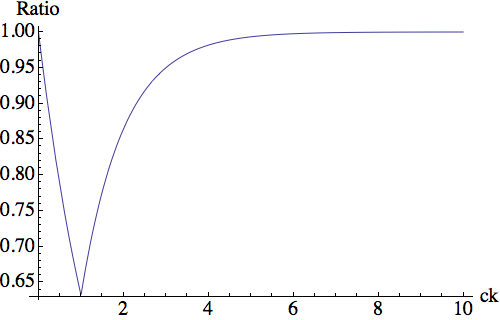
\includegraphics[width=5cm]{images/Sri_Original.png}
  \caption{Approx ratio as a function of $ck$ }\label{fig:simple_approx}
\end{minipage}
%\begin{minipage}[h]{0.45\textwidth}
%  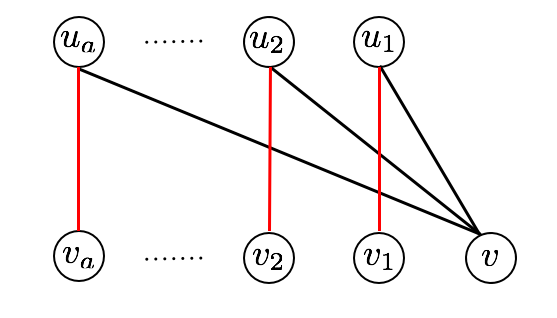
\includegraphics[width=.4\textwidth]{images/greedy.png}
%  \caption{This diagram shows one step of the greedy algorithm. When $v$ selects edges to $u_1,\ldots, u_a$, it potentially removes $v_1,\ldots, v_a$ from the pool of candidates that are avaiable. The potentially invalidated edges are shown in red.}
%\end{minipage}
\end{figure}

%Now suppose that $G$ is generated and $H$ is sampled using the same
%processes as described above. The next theorem, extends the above
%bounds to the $(c,a)$-graph recommendation problem where $a>1$.
%In particular if we set $a=1$, we will obtained the estimate from the original analysis.

%Now, we can perform a similar analysis as before. In
%particular, 
For the general $(c, a)$-recommendation subgraph problem, if $ck>a$, then the problem is easy on average. This
is in comparison to the trivial estimate of $cl$. For a fixed $a$, a
random solution gets better as $ck$ increases because the decrease in
$e^{-ck}$ more than compensates for the polynomial in $ck$ next to
it. However, in the more realistic case $ck<a$, we need to use the
trivial estimate of $ckr/a$, and the analysis for $a=1$ does not extend here. 
The following table shows how large 
$ck$ needs to be for the solution to be 95\% optimal for different
values of $a$.\vs

%In both this analysis and the previous one, $ck$ is the average degree
%of a vertex $v\in R$ in our chosen subgraph. The original analysis
%showed that if $ck>1$, then the sampling algorithm will probably cover
%every vertex in $R$ since the expected degree of each vertex is large.
%On the other hand if $ck$ is small ($ck < 1$) then the best possible
%solution is obtained when none of the vertices in $R$ has degree
%greater than 1. \vs

%If $ck<1$, then we do not cover very
%many vertices in $R$, but we also do not cover many vertices more than
%once. Since the optimal solution in this case was correspondingly low,
%our solution was good in the $a=1$ case. However, when $a<1$, the fact
%that our edges are well-dispersed only hurts our solution because we
%need to concentrate the edges on specific nodes in $R$ that will
%eventually count in the objective. 

\begin{figure}[h]
  \centering
  \begin{tabular}{ |c|c|c|c|c|c| }
    \hline
    $a$ & 1 & 2 & 3 & 4 & 5 \\ \hline
    $ck$ & 3.00 & 4.74 & 7.05 & 10.01 & 13.48 \\
    \hline
  \end{tabular}
  \caption{The required $ck$ to obtain 95\% optimality for $(c, a)$-recommendation subgraph}
\end{figure} 

We close out this section by showing that the main result that holds in expectation also hold with high probability. 
While Chernoff bounds are usually stated for independent variables, the
variant below holds for any number of pairwise non-positively correlated
variables.

\begin{thm}\label{negative_corr_chernoff}~\cite{AugerDoerr2011}
Let $X_1,\ldots, X_n$ be non-positively correlated variables. If $X=\sum_{i=1}^n X_i$, then for any $\delta\geq 0$
\[ Pr[X \geq (1+\delta)\E[X] ] \leq \left(\frac{e^\delta}{(1+\delta)^{1+\delta}}\right)^{\E[X]} \]
\end{thm}

Using this we can convert our expectation result to one that holds 
with high probability.

\begin{thm}
Let $S$ be the random variable denoting the number of vertices $v \in R$ such that $\deg_{H}(v)\geq 1$. Then
$ S \leq r(1-2\exp(-ck))$ with probability at most $(e/4)^{r(1-\exp(-ck))}$.
\end{thm}

\begin{proof}
We can write $S$ as $\sum_{v\in R} 1-X_v$ where $X_v$ is the indicator
variable that denotes that $X_v$ is matched. Note that the variables
$1-X_v$ for each $v\in R$ are non-positively correlated. In
particular, if $N(v)$ and $N(v')$ are disjoint, then $1-X_v$ and
$1-X_{v'}$ are independent. Otherwise, $v$ not claiming any edges can
only increase the probability that $v'$ has an edge from any vertex
$u\in N(v)\cap N(v')$. Also note that the expected size of $S$ is
$r(1-\exp(-ck))$ by Theorem \ref{original_result}. Therefore, we can
apply Theorem \ref{negative_corr_chernoff} with $\delta=1$ and obtain
the result.
\end{proof}
